\section{Описание алгоритма} \label{section:algorithm}

Существует большое количество методов, позволяющих решать данную задачу. Методы, основанные на GAN (генеративно-состязательных) сетях \cite{gan-1},\cite{3d-gan} и VAE (вариацонном автоэнкодировщике) \cite{adversarial-autoencoder}, \cite{3d-autoencoder},\cite{lrgm-cloud}, не могут быть применены для решения данной задачи, по причине крайне малого (для задачи глубинного обучения) размера выборки. К примеру, в работе \cite{lrgm-cloud} при обучении на одну категорию используется более 1000 объектов. Более того, далеко не все архитектуры нейронных сетей позволяют на вход передавать облака точек с разными количествами вершин. В работе \cite{lrgm-cloud} авторы принудительно ограничивают вход сети определенным количеством точек. Стоит отметить, что в данном случае, можно было бы использовать специальные свертки , чтобы преодолеть подобные ограничения. 


\subsection{Выравнивание объектов (Alignment)}

Вначале все объекты в выборке необходимо выравнить. То есть, сделать так, чтобы ориентация всех зубов была одинаковой.
Задача оптимального совместного положения геометрических объектов широко известна и хорошо изучена. В общем случае задачу можно сформулировать следующим образом: пусть у нас имеется два облака точек $A$ и $B$. Необходимо найти матрицу поворота $R$, вектор сдвига $t$ и коэффициент размера $s$, такие что при применении их к объекту $B$ значение метрики расстояния между объектами стало минимальным. Обычно говорят токльо о нахождении матрицы поворота. В общем случае мы не обговариваем о какой именно метрике идет речь.

В данной задаче возможны два случая: случай, когда имеется имеется взаимно однозначное соответствие точек двух объектов, и случай, когда его нет.

\subsubsection{Случай наличия взаимно однозначного соответствия точек двух объектов}
Пусть у нас имеются два объекта, причем для каждой точки $a_{i}$ первого объекта $A = \{a_{1}, \ldots, a_{N}\}$, существует соответствующая точка $b_{i}$ второго объекта $B = \{b_{1}, \ldots, b_{N}\}$. Наличие данного соответствия отражается в функции расстояния между объектами (из соответствующей точке первого объекта вычисляется соответствующая точка второго объекта): $D(A, B) = \sum_{k=1}^{N}  \norm{a_{k} - b_{k}}_{2}^{2}$. 

Тогда задача поиска матрицы поворота в точности является \textit{задачей Вахба (Wahba's problem)} \cite{wahba}, которая заключается в нахождении матрицы поворота $R$, минимизирующей функция ошибки \[I(\textbf{R}) = \sum_{k=1}^{N}  \norm{a_{k} - \textbf{R} \, b_{k}}_{2}^{2} \]. Также существует \textit{ортогональная задача Прокрустеса (Orthogonal Procrustes problem)}, являющаяся аналогичной поставленной задаче.

\subsubsection{Случай отсутствия взаимно однозначного соответствия точек двух объектов}

В случае отсутствия взаимно однозначного соответствия задача выглядит следующим образом: пусть у нас имеются два объекта $A = \{a_{1}, \ldots, a_{N}\}$ и $B = \{b_{1}, \ldots, b_{K}\}$. Требуется найти такую матрицу $R$, чтобы функция ошибки \[I(\textbf{R}) = \sum\limits_{a \in A} \norm{a - \textbf{R} \, \textit{closest}(a, B)} \], где $\textit{closest}(a, B) = \argmin\limits_{b_{1}, \dots , b_{K}} \norm{a - b}$ принимала минимальное значение.


Данная задача в точности является задачей выравнивания множест точек (point set registration, point). Данная задача хорошо изучена и существуют различные алгоритмы для ее решения.


\subsubsection{Выбор алгоритма}
Так-как в выборке нету однозначного соответсвтия точками (более того, объекты выборки имеют разные количества врешин), то мы будем использовать rigid-ICP алгоритм. Самой простой версии алгоритма оказалось достаточно и в дальнейшем мы ее просто будем называть ICP.

Размер является важной частью формы элемента зуба, которую нельзя игнорировать (то есть, нельзя просто усреднить все зубы). При этом объекты в выборке для каждого типа зуба различаются по размерам (в ширину, в высоту, в длину) не более чем в полтора раза, 


\subsection{Нахождение общего порядка точек}

В дальнейших шагах алгоритма нам понадобится иметь общий порядок точек для всех облаков, то есть требуется найти взаимнооднозначное соответствие между вершинами облаков точек. Предыдущий шаг, во многом был нужен именно для того, чтобы процедура поиска соответствющий точек выполнялась как можно точнее. 


Для этого, мы выбираем из выборки облако точек с наименьшим количеством вершин (все равно больше соответствий мы найти не сможем). Если такие объектов будет несколько, то выбираем среди них один случайным образом. Будем называть найденное облако точек \textit{референсным}.


Теперь опишем процедуру поиска соответствия между вершинами для двух облаков точек. Пусть на вход передаются два облака точек, причем второе имеет меньше либо равное количество вершин чем первое облако. Для каждой вершины во втором облаке мы ищем ближайшую к нему вершину в первом облаке, и ставим их в однозначное соответствие. Разумеется, что часть точек первого облака мы потеряем, более того, возможно, что нескольким разным вершинам из второго облака будут соответствовать одинаковые вершины из первого.


Выполним описанную выше процедуру для каждого объекта из выборки и референсного облака. Теперь, у нас есть взаимно однозначные соответствия вершин для всех облаков в выборке. 

В итоге, мы задаем некоторый случайный порядок вершин на референсном облаке, и, имея взаимно однозначное соответствие вершин для всех объектов из выборки, мы получаем порядок и для всех облаков в выборке.

Несмотря на то, что данный подход весьма прост, на имеющейся выборке он показывает хорошие результаты (в данном случае, большую роль играет выровненность объектов и их однородность).

% УВЕЛИЧЕНИЕ ОБЪЕМА!! придумать и вставить картинку

\subsection{Снижение размерности и анализ главных компонент}

\begin{figure*}[ht!]
    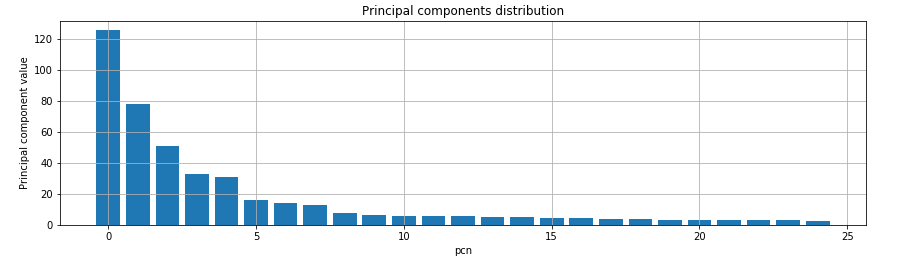
\includegraphics[width=1\linewidth]{images/pcd-example.png}
	\caption{Пример распределения значений главных компонент}
    \label{fig:pcd-ex}
\end{figure*}


\subsection{Генерация новых объектов}


